\documentclass{article}
% \usepackage{graphicx}
\usepackage{amsmath}
\usepackage{amsfonts}
% \usepackage[parfill]{parskip}
\usepackage{hyperref}
% \usepackage[useregional]{datetime2}
% \usepackage[toc,page]{appendix}

\usepackage{biblatex}
\addbibresource{references.bib}

% Use \lstset to make myStyle the global default
% \lstset{style=myStyle}

% \graphicspath{ {./figures/} }

\title{ELEC-E5510: Speech Recognition\\
    \large Literature Study Report: Multi-modal Emotion Recognition}

% \newcommand{\inlinemaketitle}{{\let\newpage\relax\maketitle}}

\def\sectionautorefname{Section}

\begin{document}

\maketitle
% \tableofcontents
% \newpage

% \listoffigures
% \newpage

% Content of report would be written here
% \include{./tex/task1.tex}
% ...
% \include{./tex/task2.tex}

%%% Motivation of Emotion Recognition
Computers, or machines in general, are becoming more and more integrated into our daily lives.
They are used in various applications, such as in healthcare, education, and entertainment.
In many of these applications, it is important for the machine to be able to understand the
emotional state of the user. For example, in healthcare, a machine that can recognize the
emotional state of a patient can provide better care and support. In education, a machine
that can recognize the sentiment of a student can provide personalized learning experiences.
In other words, emotion recognition in real time is essential for human-computer interaction.
Many studies have been conducted to develop systems that can recognize human emotions from
data collected from various sources, such as facial expressions, speech, text and physiological
signals. Among them, physiological signals are more objective and reliable than other sources
~\cite{unimodal-to-multimodal}.
Human emotions can be classified into six fundemental expressions: happiness, sadness,
fear, anger, disgust, and surprise. Other variant emotions can be derived from these six
basic emotions~\cite{basic-emotions}.

%%% Motivation and introduction to  multimodal emotion recognition
An unimodal emotion recognition system uses data from a single source from the
aforementioned sources to recognize emotions. However, in order to improve the accuracy of
emotion recognition, researchers have started to explore the use of multimodal data, which
combine data from multiple sources. It has been shown that multimodal emotion recognition
is superior to unimodal emotion recognition, as it can capture more information about the
emotional expression~\cite{multimodal-review, unimodal-to-multimodal}. Due to the
simplicity and efficiency of deep learning models, they have been widely used in multimodal
emotion recognition systems~\cite{multimodal-review, unimodal-to-multimodal}. They
especially excel in high-level feature extraction for facial images and text.
According to~\cite{multimodal-review},
there are three fundemental multimodal fusion methods for emotion recogintion:
\begin{itemize}
    \item Feature-level fusion: Features from different modalities are concatenated and fed into a classifier.
    \item Decision-level fusion: Classifiers are trained separately for each modality,
    and the outputs are combined using a fusion rule.
    \item Hybrid fusion: A combination of feature-level and decision-level fusion.
\end{itemize}
Feature-level fusion is the most commonly used method in deep learning-based
multimodal emotion recognition systems due to ability to integrate rich, complementary information
from multiple modalities, enhancing model accuracy by capturing subtle cross-modal emotional
cues early in the processing pipeline~\cite{multimodal-review}.


\printbibliography[heading=bibintoc]

% \newpage
% \begin{appendices}
%     \section{Code}
All code is publicly accessible at \url{https://github.com/ancuongnguyen07/Multimodal-ERC/tree/master/code}

\begin{lstlisting}[label={lst:training-script},caption=Running the training script.]
python train_MELD.py --features-type text_audio_visual \
    --data-path data/MELD_features_raw1.pkl --output-dir models/
\end{lstlisting}

\begin{lstlisting}[label={lst:testing-script},caption=Running the testing script.]
python test_MELD.py --model-path ../models/text_audio_visual_BiDi_Att.pth \
    --features-type text_audio_visual
\end{lstlisting}

\section{Confusion Matrices}
\begin{figure}[htbp]
    \centering
    \begin{subfigure}[b]{0.45\textwidth}
        \centering
        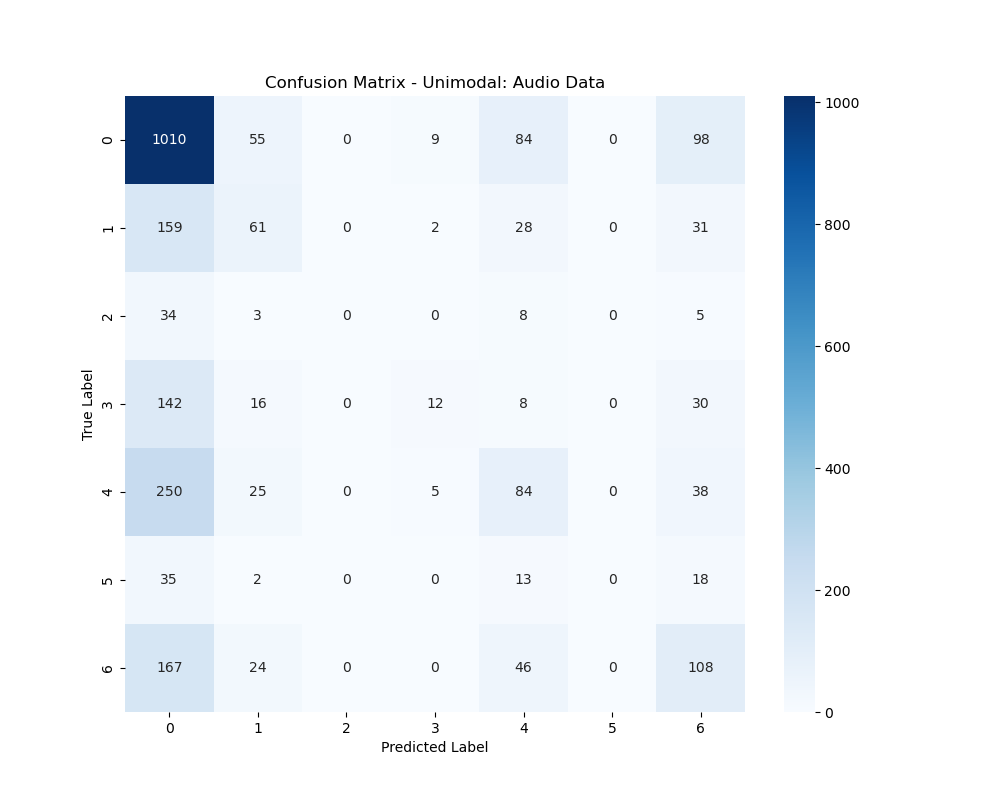
\includegraphics[width=\textwidth]{figures/audio.png}
        \caption{Unimodal: Audio Data}
    \end{subfigure}
    \hfill
    \begin{subfigure}[b]{0.45\textwidth}
        \centering
        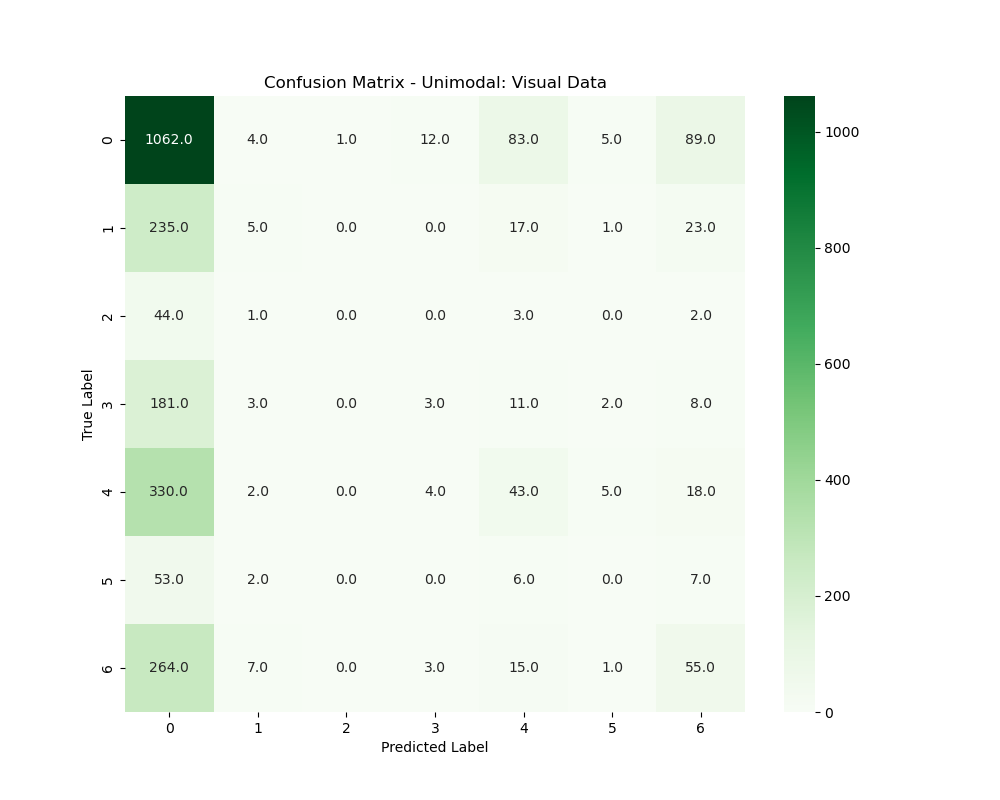
\includegraphics[width=\textwidth]{figures/visual.png}
        \caption{Unimodal: Visual Data}
    \end{subfigure}

    \vspace{0.5cm} % Vertical space between rows

    \begin{subfigure}[b]{0.45\textwidth}
        \centering
        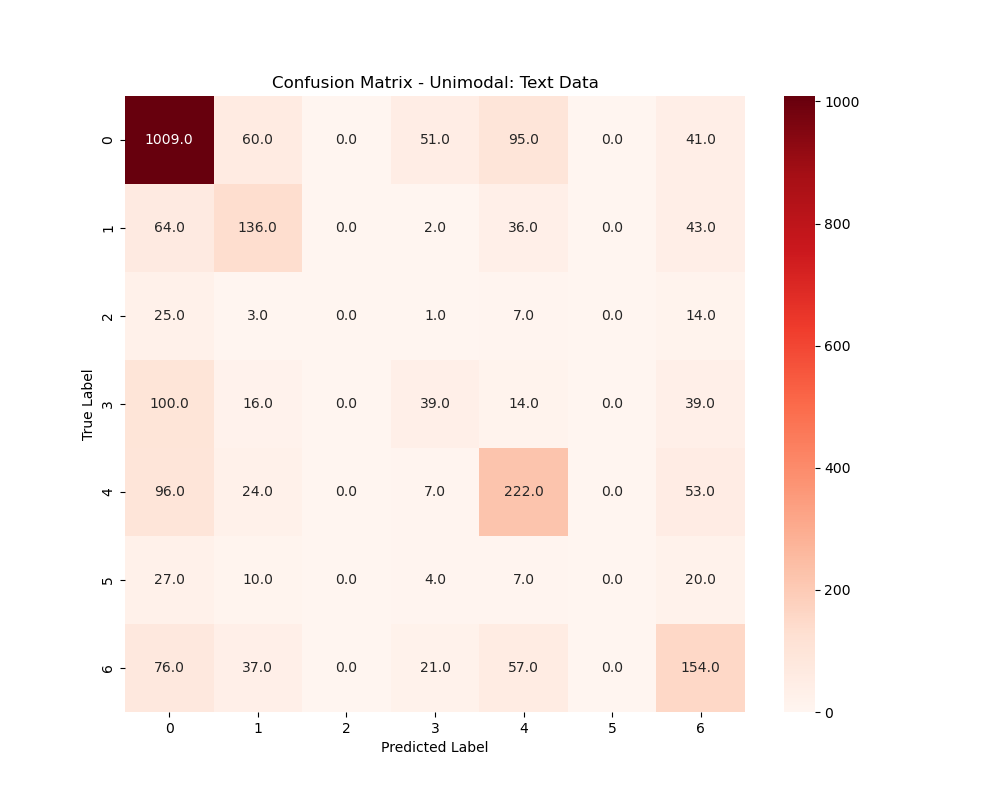
\includegraphics[width=\textwidth]{figures/text.png}
        \caption{Unimodal: Text Data}
    \end{subfigure}
    \hfill
    \begin{subfigure}[b]{0.45\textwidth}
        \centering
        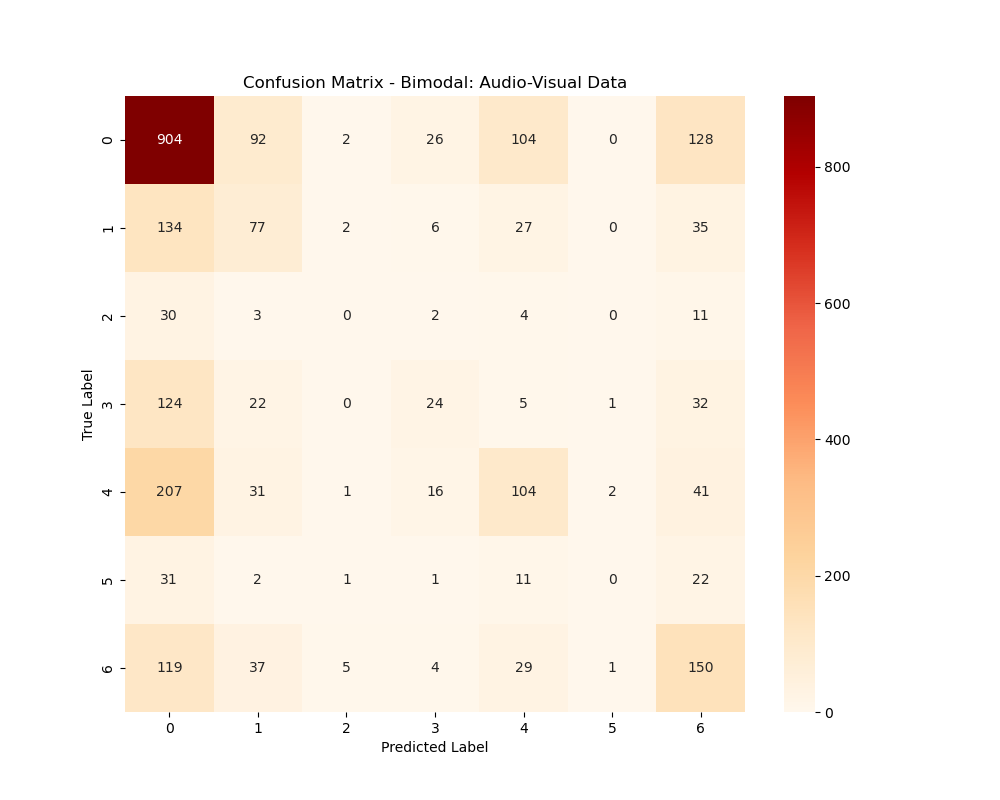
\includegraphics[width=\textwidth]{figures/audio-visual.png}
        \caption{Bimodal: Audio-Visual Data}
    \end{subfigure}

    \vspace{0.5cm} % Vertical space between rows

    \begin{subfigure}[b]{0.45\textwidth}
        \centering
        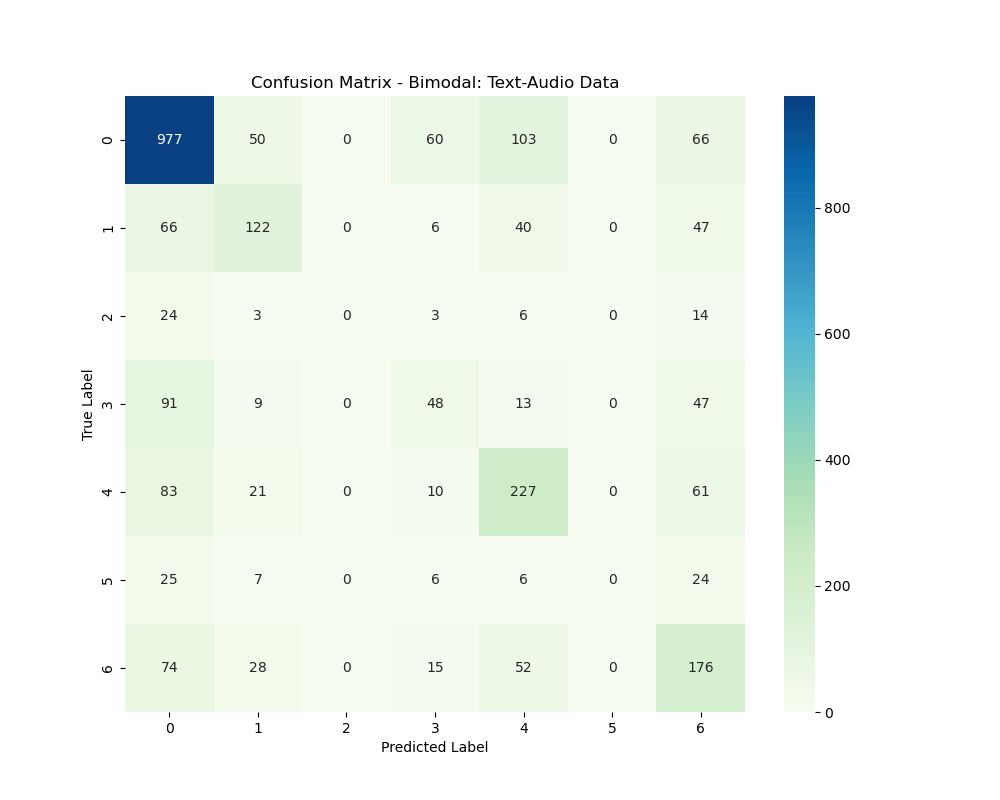
\includegraphics[width=\textwidth]{figures/text-audio.png}
        \caption{Bimodal: Text-Audio Data}
    \end{subfigure}
    \hfill
    \begin{subfigure}[b]{0.45\textwidth}
        \centering
        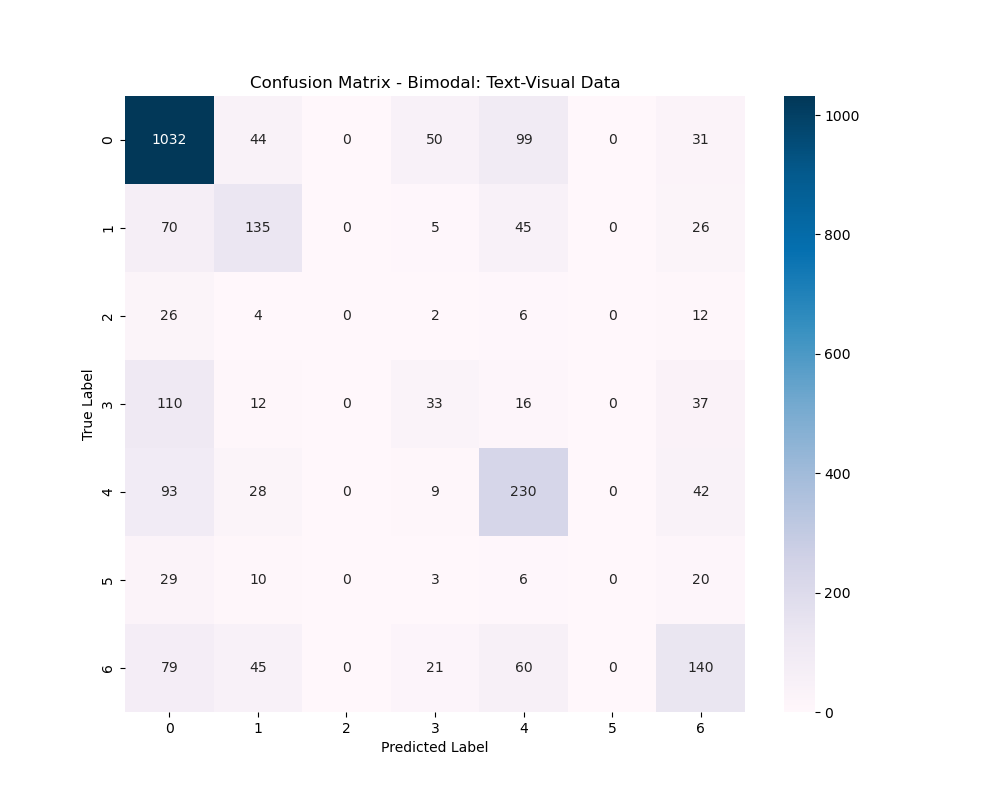
\includegraphics[width=\textwidth]{figures/text-visual.png}
        \caption{Bimodal: Text-Visual Data}
    \end{subfigure}

    \vspace{0.5cm} % Vertical space between rows

    \begin{subfigure}[b]{0.45\textwidth}
        \centering
        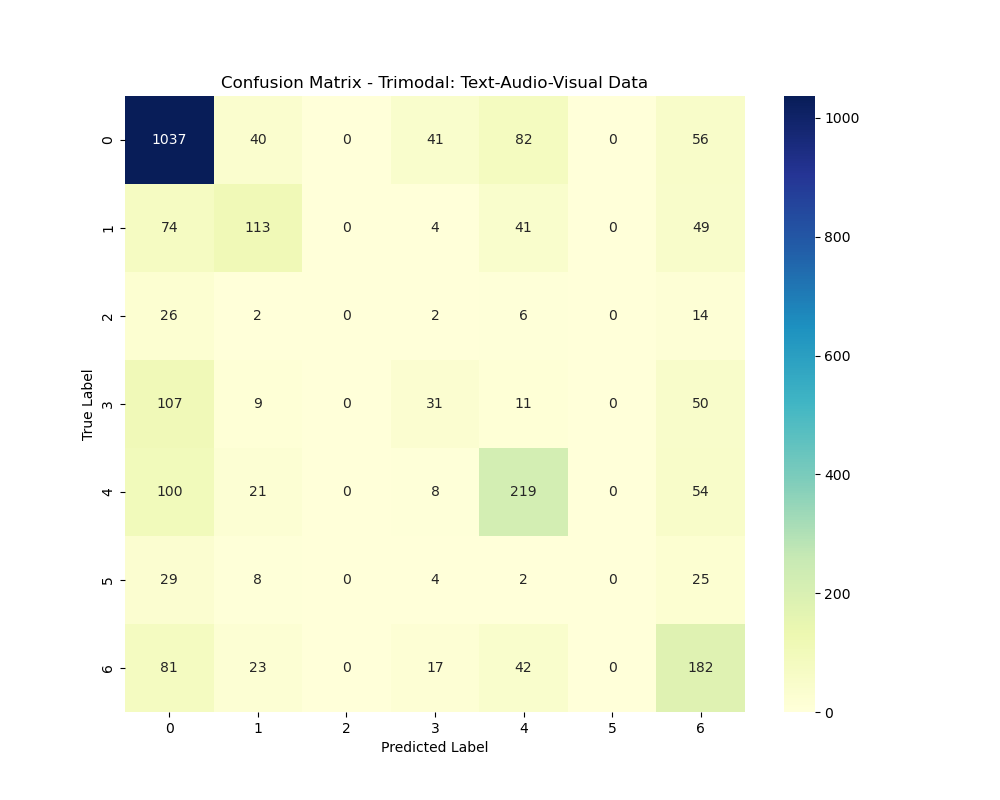
\includegraphics[width=\textwidth]{figures/text-audio-visual.png}
        \caption{Trimodal: Text-Audio-Visual Data}
    \end{subfigure}

    \caption{Confusion Matrices Across Modalities}
    \label{fig:confusion_matrices}
\end{figure}
% \end{appendices}

\end{document}
